\documentclass[a4paper]{article}
\usepackage{listings}
\usepackage{qtree}
\usepackage{xcolor}
\usepackage{forest}
\usepackage{multicol}
\setlength{\columnsep}{3cm}
\usepackage{parskip}
\usepackage{changepage}
\usepackage[T1]{fontenc}
\usepackage{amsmath}
\usepackage{hyperref}
\usepackage{listings}
\usepackage{amsthm}
\usepackage{amssymb}
\usepackage{float}
\usepackage[utf8]{inputenc}
\usepackage{graphicx}
\usepackage[italian]{babel}
\usepackage{thmtools}
\graphicspath{{figures/}}

\begin{document}

\author{Lorenzo Dentis, lorenzo.dentis@edu.unito.it}
\title{Esercizio finale}
\maketitle

\subsection{Introduzione}
L’esercizio consiste nella verifica di 3 proprietà in diverse varianti di un algoritmo di mutua esclusione presentato sul libro a partire dall’algoritmo 3.2 fino all’algoritmo 3.10 denominato Algoritmo di Dekker.
Le 3 proprietà da verificare sono:
\begin{itemize}
	\item \textbf{Assenza di deadlock}: Se qualche processo cerca di accedere alla regione critica eventualmente un processo potrà farlo.
	\item \textbf{Mutua esclusione}:  le istruzioni delle sezioni critiche di due o più processi non possono essere eseguite in modo interfogliato.
	\item \textbf{Assenza di starvation individuale}: Se un processo cerca di accedere alla regione critica eventualmente quel processo potra' farlo.
\end{itemize}

\section{Algoritmo 3.2}
\label{SEC:3.2}
\begin{center}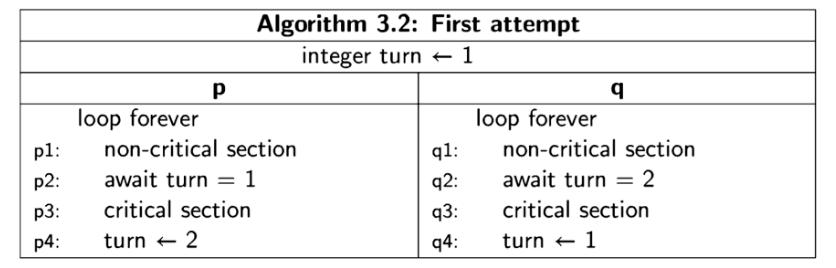
\includegraphics[width=1\textwidth]{3.2.png}\end{center}
Questo primo algoritmo propone la mutua esclusione tramite una singola variabile \textit{turn} che identifica quale processo tra \textit{p} e \textit{q} può accedere alla regione critica.
Questo algoritmo rispetta i criteri di \textbf{Assenza di deadlock \textbf{e} Mutua esclusione} ma non garantisce l' \textbf{Assenza di starvation individuale}
\newpage
\subsection{Rete di Petri}
In questo particolare caso è stato possibile effettuare una composizione Name-based \ref{FIG:3.2PN}.
\begin{figure*}[!ht]
\centering
\makebox[\textwidth][c]{
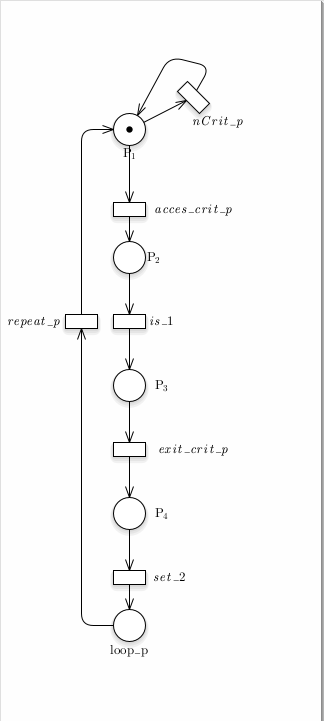
\includegraphics[width=0.5\textwidth]{p3.2.png}
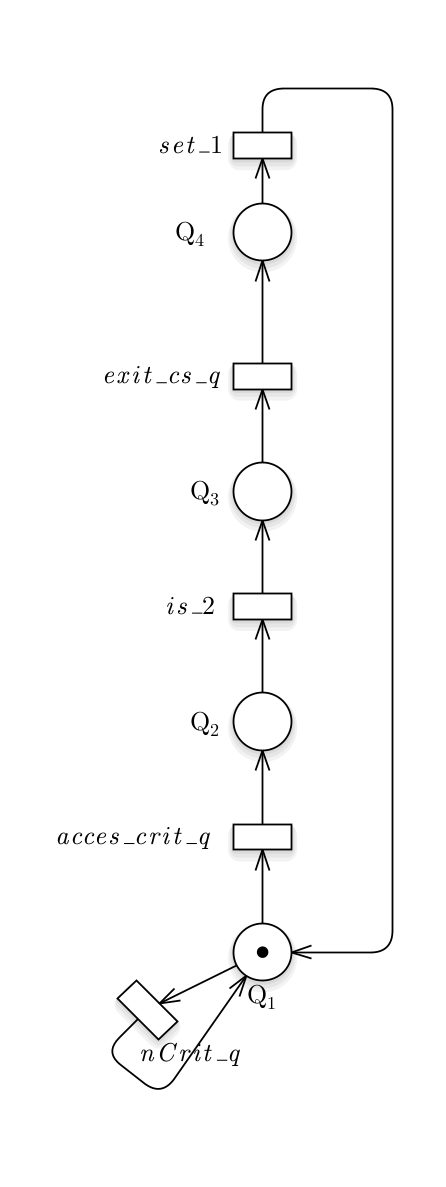
\includegraphics[width=0.5\textwidth]{q3.2.png}
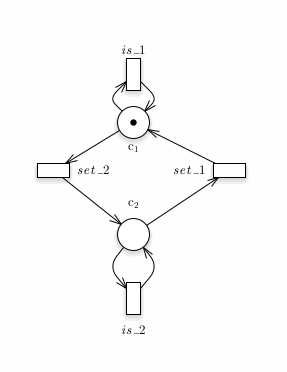
\includegraphics[width=0.5\textwidth]{variable3.2.png}}
\caption{Rete di petri decomposta} \label{FIG:decomposed3.2PN}
\end{figure*}
\begin{figure*}[!ht]
\centering
\makebox[\textwidth][c]{
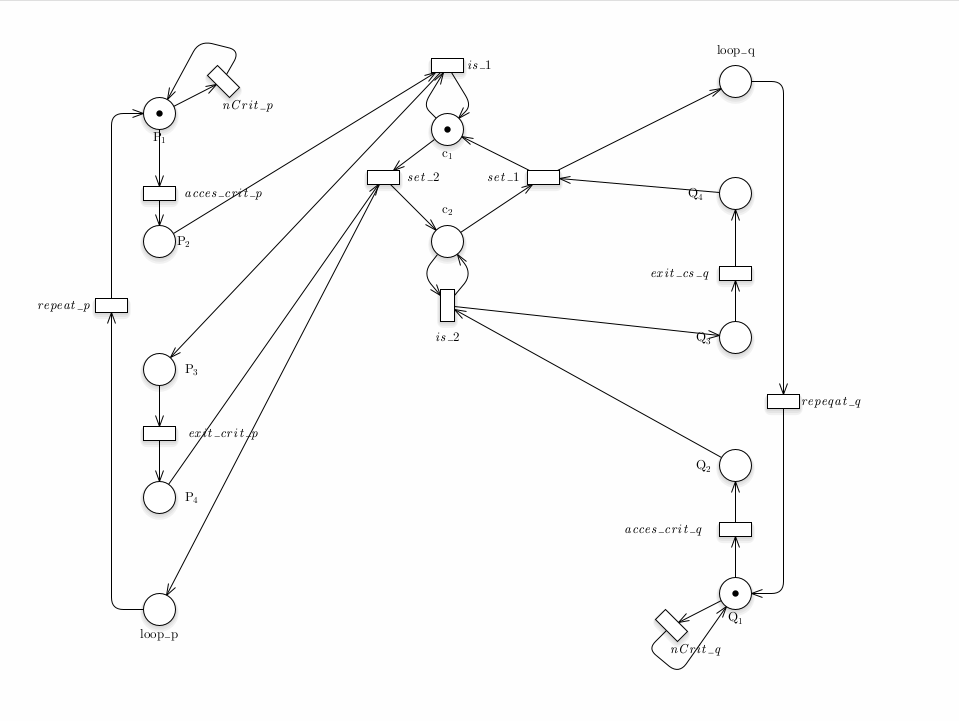
\includegraphics[width=1\textwidth]{3.2PN.png}}
\caption{Rete di petri composta} \label{FIG:3.2PN}
\end{figure*}
\newpage
\subsubsection{RG}
Il reachability graph, in figura \ref{FIG:3.2RG}, è composto da 30 stati raggiungibili e non presenta alcun deadlock.
\begin{figure*}[!ht]
\centering
\makebox[\textwidth][c]{
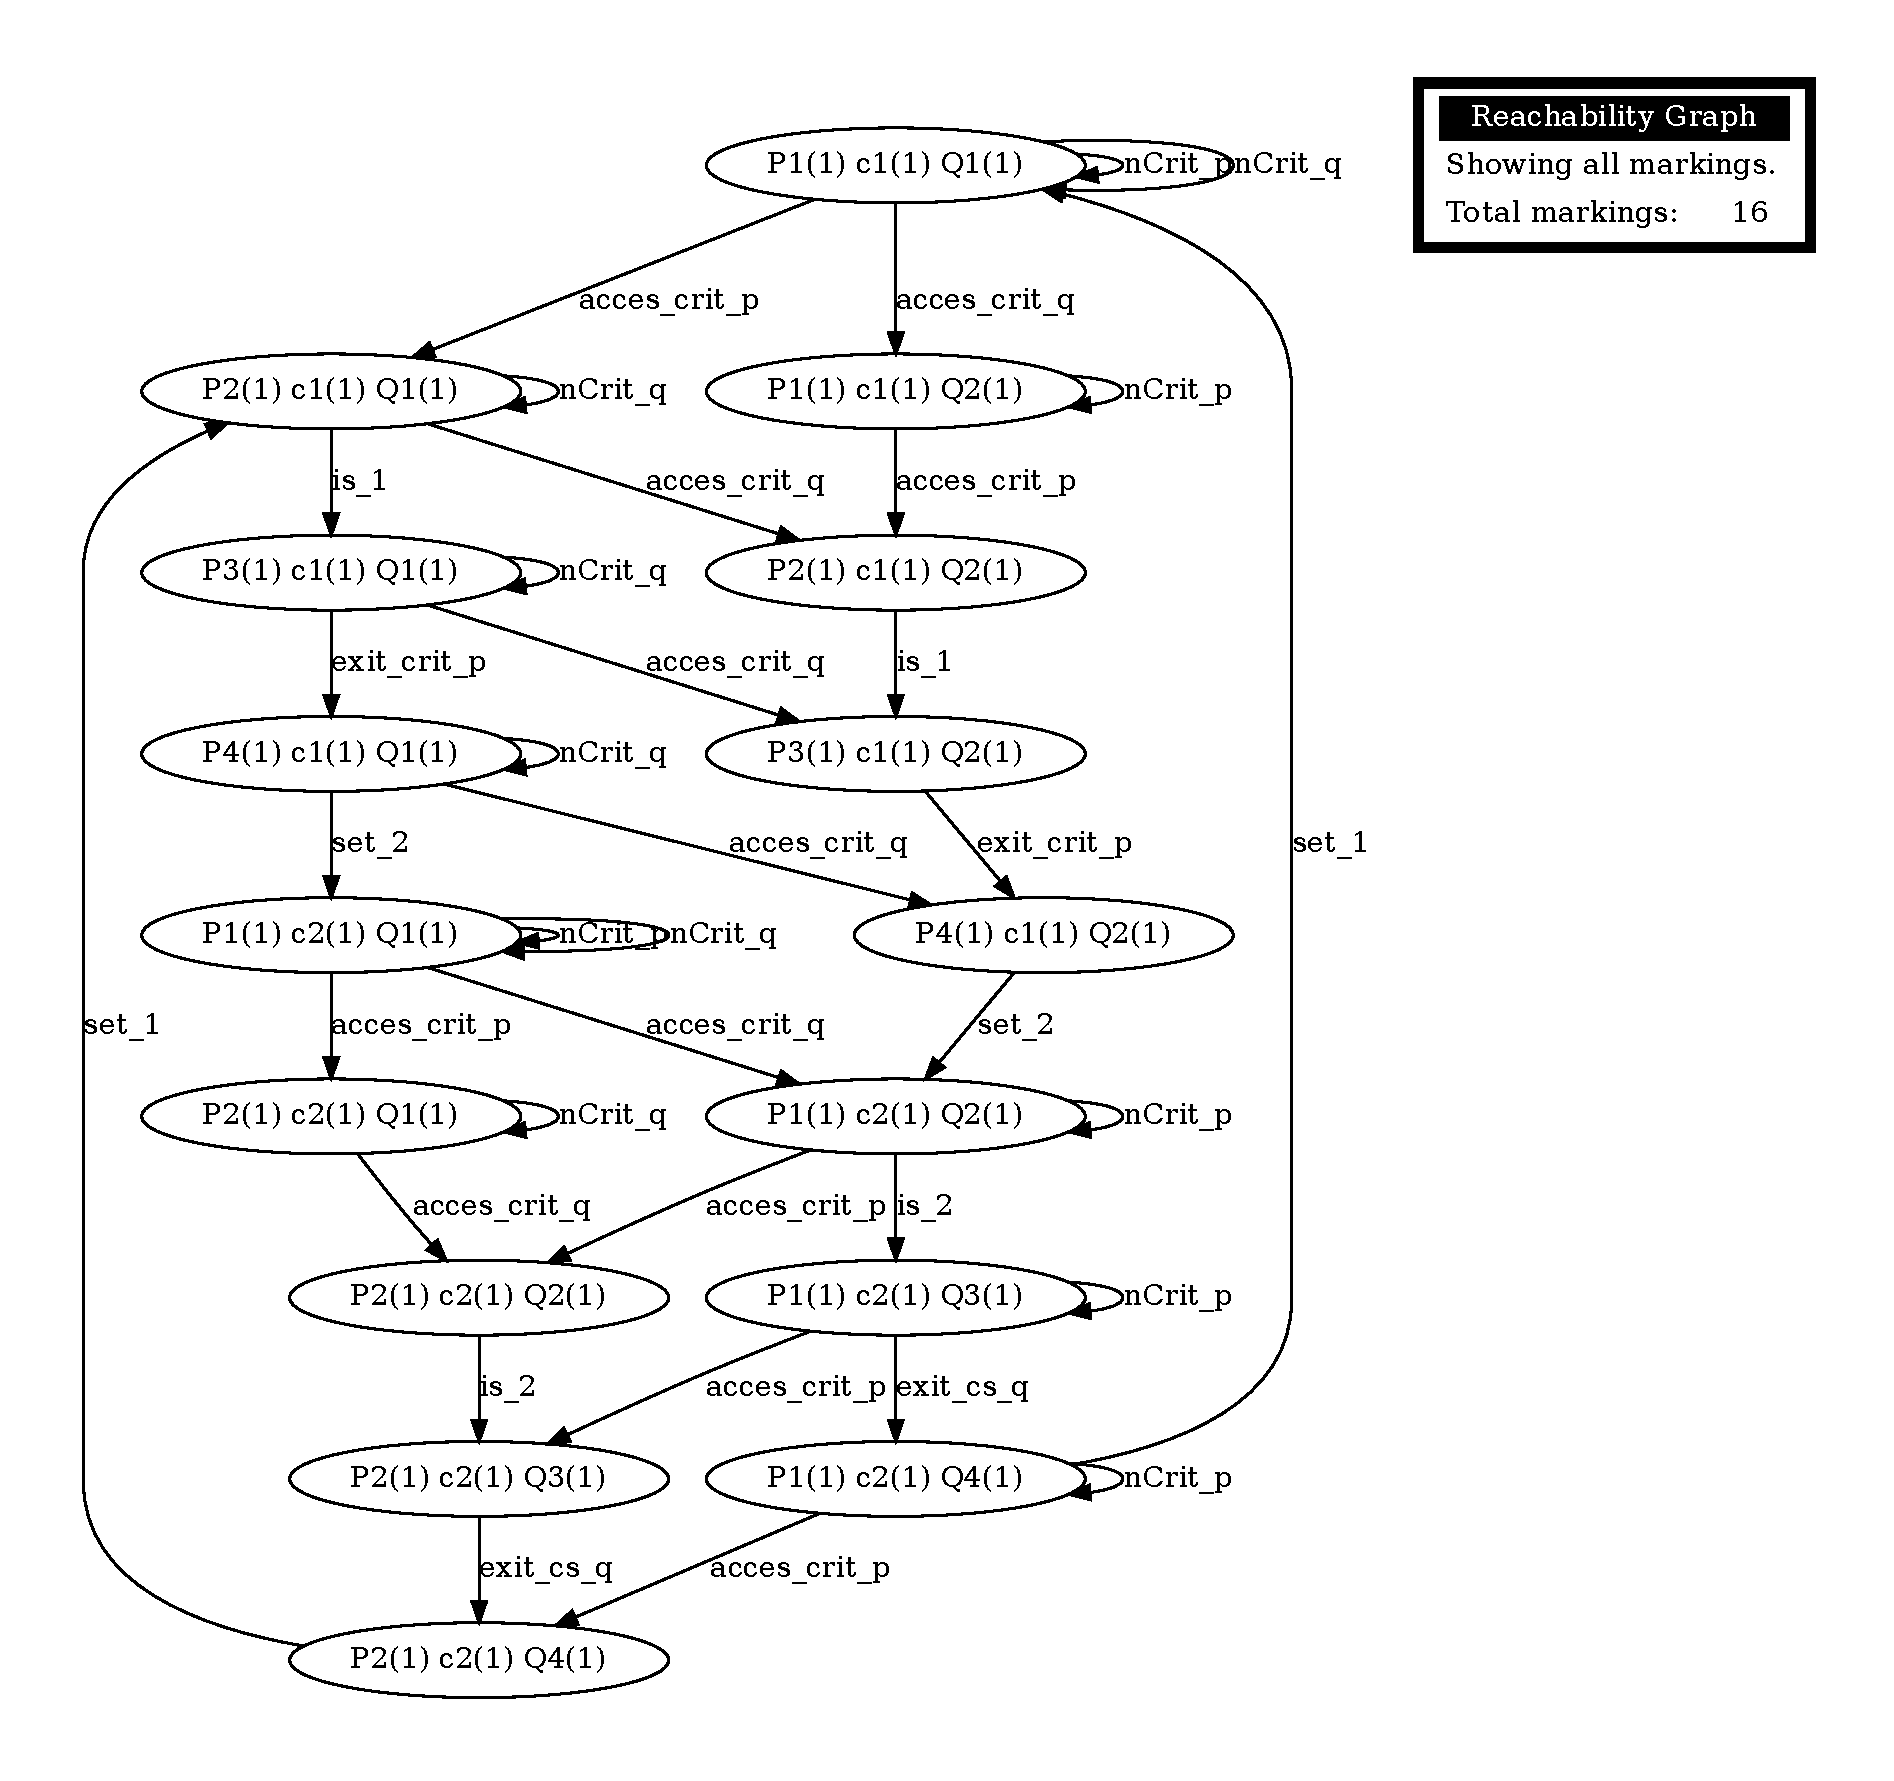
\includegraphics[width=1\textwidth]{3.2RG}}
\caption{Reachability graph 3.2} \label{FIG:3.2RG}
\end{figure*}
\newpage
\subsubsection{Analisi strutturale}
Il calcolo dei \textit{semiflow} fornisce 3 \textit{T-semiflow} minimali e 3 \textit{P-semiflow} minimali, i 3 \textit{P-semiflow} permettono di produrre dei P-invarianti e di studiare la boundedness, che in questo caso rivela che tutti i posti sono 1-bound.
Invece dallo studio dei \textit{T-semiflow} si può affermare che il sistema possiede la proprietà di \textit{liveness} in quanto è possibile individuare una \textit{firing sequence} attivabile dalla marcatura iniziale che riporta ad una situazione analoga alla situazione iniziale.
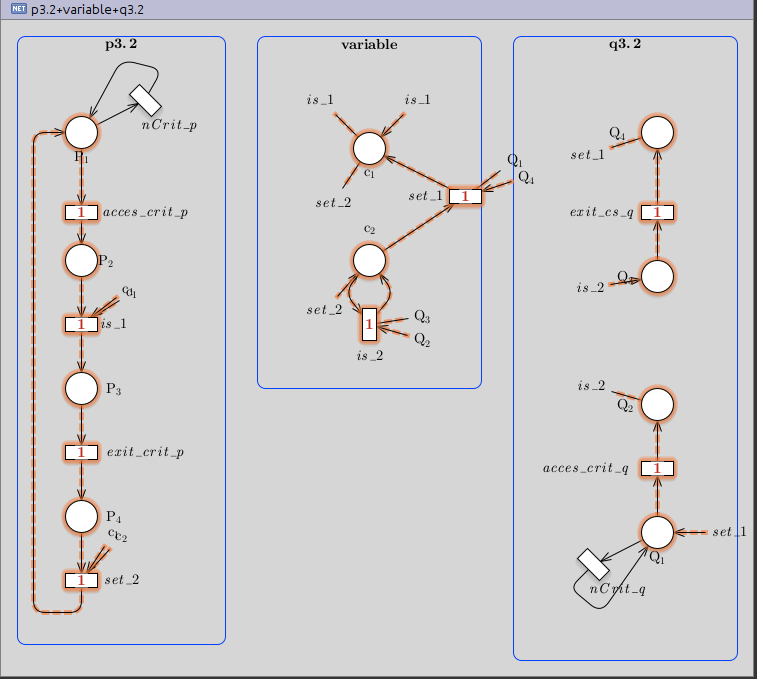
\includegraphics[width=1\textwidth]{3.2T.png}

\subsubsection{model checking}

\subsection{Algebra dei processi}
La codifica del sistema in CCS risulta essere: 
\begin{flalign*}
	&SYS = (P_1 || Q_1 || T_1) /_{\{isT_1, setT_1, isT_2, setT_2\} }&&\\
	&P_1=ncsP_1 + ncsP.P_2&&\\
	&P_2=isT_1.P_3&&\\
	&P_3=csP.P_4&&\\
	&P_4=setT_2.P_4&&\\
	&Q_1=ncsQ_1 + ncsQ.Q_2&&\\
	&Q_2=isT_2.Q_3&&\\
	&Q_3=csQ.Q_4&&\\
	&Q_4=setT_1.Q_4&&\\\\
	&T_1=\overline{isT_1}.T_1 + \overline{setT_2}.T_2&&\\
	&T_1=\overline{isT_2}.T_2 + \overline{setT_1}.T_1&&\\
\end{flalign*}
Da cui segue il seguente derivation graph (in cui la riduzione è omessa per chiarezza).\\
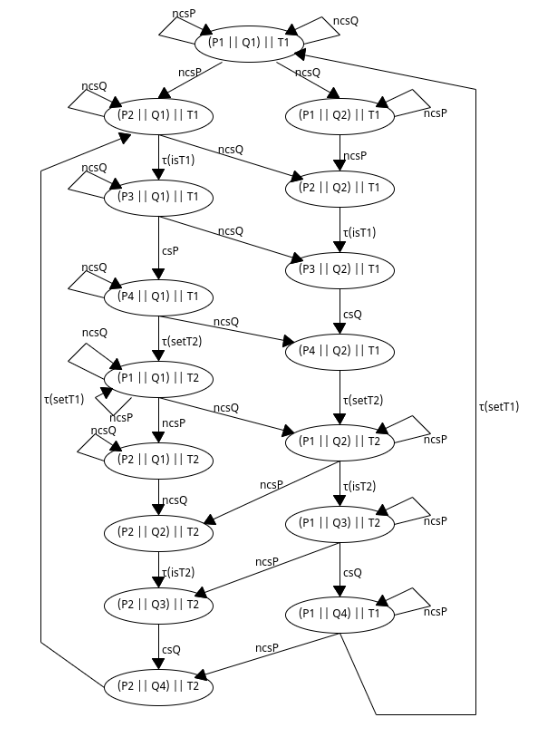
\includegraphics[width=1\textwidth]{3.2CCS.png}\\
Come si può notare il \textit{DG} è composto da 16 stati, esattamente il numero di stati raggiungibili del Reachability Graph, questo è un risultato aspettato in linea con quanto analizzato nelle corrispondenti parti dell'esercizio produttore-consumatore.

\subsection{NuSMV}
L'implementazione del sistema tramite il linguaggio di NuSMV sfrutta la similarità che c'è tra il processo P ed il processo Q.
Infatti i due programmi svolgono le stesse identiche operazioni, ma su variabili differenti, quindi basta dichiare i processi andando ad inserire correttamente i parametri.
Quindi ad esempio il processo p avrà 4 stati: lo stato s1 da cui potrà proseguire richiedendo la sezione critica, oppure rimanendo in s1, lo stato s3 che corrisponde alla sezione critica e lo stato s4 che corrisponde all'uscita dalla sezione critica ed la ripetizione del programma completo.\\
Più interessante è lo stato s4, dove si nota il riuso del codice. 
Per poter accede alla sezione critica il turno deve essere 1, quindi il processo P va a confrontare il valore della variabile \textit{turn} con lo il valore della variabile \textit{var\_wait} che in questo caso è 1, se corrispondono il programma prosegue in s3.
Operazione simile viene effettuata quando P va ad impostare il valore della variabile \textit{turn} in uscita dalla sezione critica.
\lstinputlisting{figures/3_2.smv}
Il comando \texttt{print\_reachable\_states} mostra 16 stati raggiungibili di 32 possibili, in linea con la dimensione del Derivation Graph e del Reachability Graph.
Tra tutti gli stati raggiungibili non è presente alcuno stato di Deadlock.

\subsubsection{Model Checking NuSMV}
\end{document}
